\chapter{Methodology}
\label{ch:method}
\section{...}
As previously mentioned, I am going to be using the CRISP-DM model (\cite{WirthCRISP-DM:Mining}) to break down the problem into 6 specific stages \textbf{reference the figure from intro} 


\section{Business Understanding}

This sections asks the question of what exactly the business needs and hopes to gain from the process, in this case the business needs to gain a better understanding of which customers are most likely to cancel there bookings. Doing this will help to not only prevent bookings from being cancelled but also to gain a better overall understanding of why bookings are cancelled. It is also important form a machine learning and a business perspective to understand why bookings are being cancelled through the process of feature and model explanation as this will help to understand what the best actions are that can be taken to prevent cancellations.

\begin{figure}[hbt!]
 %\centering
 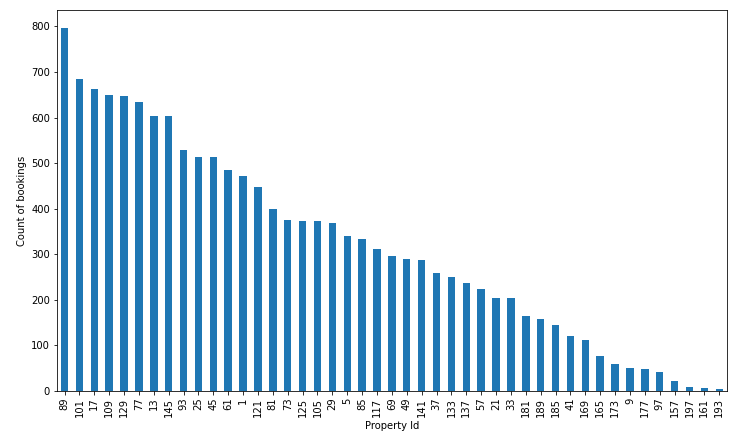
\includegraphics[width=10cm]{figures/bookings_by_property.png}
 \caption{The X axis shows each of the property Ids with the Y axis showing the total number of bookings made}
\end{figure}



In total the dataset contains 45 properties, that vary significantly in the number of students at each of them \textbf{as shown in figure 1} because of this large variation I think it will be best to understand cancellations at the global level with one model being trained on data from all properties. Doing this helps to prevent model over fitting as with a relatively small number of data points on some of the properties it would be difficult to create an accurate model. The risk involved with this is that the model will not pickup some of the discrepancies between the individual properties. 

\begin{itemize}
\item Determine data mining goals - Understanding the dataset in question in essential to being able to properly evaluate and understand its results - \textbf{explain this better}
\end{itemize}





\section{Data Understanding}

To get the relevant data for solving this problem I first had to approach the wider problem of developing a robust data warehouse [\textbf{reference}] I started by building a dynamic data stream that could take data from an external source and store it in the company data warehouse so I would be able to run new iterations of the model as new data came in. To facilitate the problem of having a dynamic data import stream I used the python object relation mapping library \cite{SQLAlchemyPython} since it has direct support for the python data library pandas \textbf{reference?}. Doing this allows me to read data in any supported format [supported formats] and store it in a SQL database with the correct data types. The data I need is stored in an Amazon S3 bucket, so I used the python S3 library Boto3 to read TSV files from blob storage every hour and stored them in the data warehouse. I then deployed this process onto a docker container using the Azure cloud tool called Container Instances that enables docker containers to run as scheduled tasks. Docker containers are standardised units of software that contain all of the dependencies for running a specific program or script in a single executable package which can be run in the cloud or on a local machine.

The booking data relevant to this problem is created in an external system, this is the website front facing to the customers where each of the bookings are taken. As a booking is made through the website customer details are stored in the external website databases. This data includes personal information of the customer like name, address, date of birth and phone number. As the customer moves further through the booking process they are then taken to a page asking which university they will be attending and to make a selection of the property they want to rent. Here information like location of property, room name, price and extras are stored. When a student then selects a specific room they will be asked about the payment structure they want to use and how they will make there deposit. It is here that all of the relevant cost data is stored. In some cases the fields for data entry are not mandatory in the booking system meaning that the data will not be stored, in these cases the value of the attribute is replaced with other.

\vspace{5mm}

The information stored within these stages of the booking describes all of the intellectual property stored about each specific customer and therefore is what will be used to predict the activity of the customer and weather or not they will cancel there booking. In the case of a classification problem we can consider any attribute relevant if it influences the target variable. With the common goal in machine learning to obtain as much useful information as possible since \textbf{[reference good number of data points for machine learning]}

In this case I will be looking only at data from the years 2020 to 2021 since the old data is incomplete. During this booking cycle there are a total of around 14363 thousand bookings.

\begin{figure}[hbt!]
 %\centering
 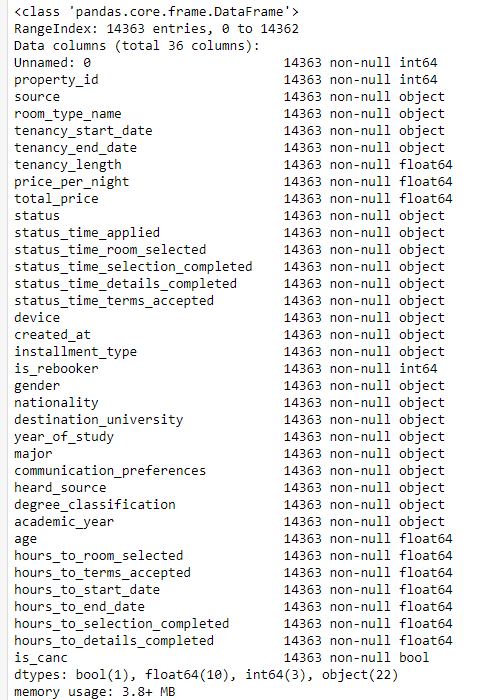
\includegraphics[width=10cm]{figures/df_info.png}
 \caption{Shows all of the attributes in the dataset}
\end{figure}


\begin{itemize}
    \item property id is the unique identifier for the residence 
    \item source is the internal system used to create the booking
    \item room type name is the category of room selected
    \item tenancy start date is the proposed start date of the contract
    \item tenancy end date is the proposed end date of the contract
    \item tenancy length is the duration in day the contract is valid for
    \item price per night is the daily rate at which the room will be sold
    \item total price is the total price for the contracted time
    \item status is the current status of the booking
    \item status time applied is the time the booking process was started
    \item status time room selected is the time the customer selected there room
    \item status time selection completed is the time the customer finalised the selected process 
    \item status time details completed is the time all personal details are entered
    \item status time terms accepted is the time the agreement is completed
    \item device is the type of the device the booking was made on
    \item created as is the time the process was started
    \item installment type is the payment schedule
    \item is rebooker defines if the same customer has applied before
    \item date of birth of the customer
    \item gender of the customer
    \item nationality of the customer
    \item destination university is the university the customer expects to go to
    \item year of study is the academic year  the customer is in
    \item major is the degree type of the student
    \item communication preference is the customer selected method of communication
    \item heard source is where the customer discovered the booking
    \item degree classification is the degree type of the customer
    \item academic year
 

\end{itemize}

 \begin{figure}[hbt!]
 %\centering
 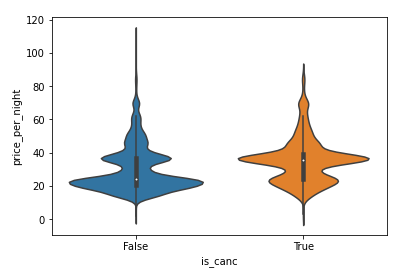
\includegraphics[width=10cm]{figures/price_per_night.png}
 \caption{Distribution of price per night comparing cancelled and non cancelled bookings}
\end{figure}
 
 
 Comparing price per night when looking at bookings that canceled to ones that didn't we can see that around the middle price range of £40 per night is where the most significant number of booking cancellations occur, with most of the non canceled bookings in the £20 per night price range. This difference in price distribution when comparing cancelled to non cancelled bookings suggests price per night is an important feature for classification. 
 
 \begin{figure}[hbt!]
 %\centering
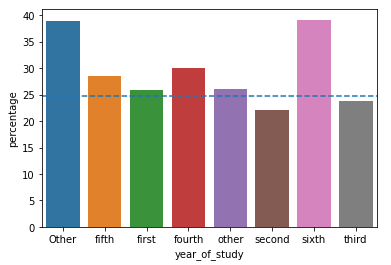
\includegraphics[width=10cm]{figures/canc_per_year.png}
 \caption{Normalized percentage of booking cancellation for degree year of study with blue horizontal line being the average}
\end{figure}
 
  
Sixth year students are more likely to cancel than any other year, possibly because they are more likely to decide to live in private accommodation but it is unlikely this accounts for them being almost twice as likely to cancel than the average. The Other category is also an outlier here with an almost 40 percent chance of cancelling, more research would be needed to understand exactly why customers who don't enter a year of study are more likely to cancel but it is clear from this figure that year of study will be a good indicator of cancellations.
  
  \begin{figure}[hbt!]
 %\centering
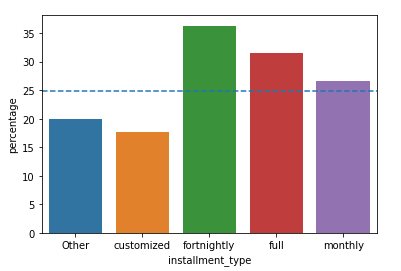
\includegraphics[width=10cm]{figures/instalment_type.png}
 \caption{Normalized percentage of booking cancellation for payment installment type}
\end{figure}
  
  
  Weighted average of cancellations looking at the selected instalment type. Instalment type is the payment plan the student selected, we can see that students who selected the fortnightly plan are 10 percent more likely to cancel than the average and students who opted for the customized installment plan are around 6 percent less likely to cancel. this may be a good predictor of cancellations.
  
  
   \begin{figure}[hbt!]
 %\centering
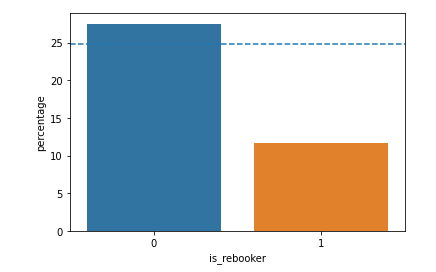
\includegraphics[width=10cm]{figures/is_rebooker.png}
 \caption{Normalized percentage of booking cancellation for rebooker}
\end{figure}
  
 Comparison in cancellations with students who are rebookers (have booked before), we can see that students who have booked previously are around half as likely to cancel there bookings. this is another good predictor of cancellations.  
  

\section{Data Preparation}

The dataset I have selected to be used for this research is a combination of 3 different tables from the external booking system, these include the booking table, student table and academic year id table. All of these tables have been combined using the data warehouse to create the DataFrame shown in \textbf{figure 3.7}. Many of the columns from the original dataset have been taken out this stage as I did not believe they would provide any value in terms of the prediction. Using a dataset with too many columns has to potential to result in over fitting and noise in the model, it is possible that the dataset I have selected can be reduced to a smaller number of features but I believe I have selected the best dataset available to me for completing this research. 

\begin{figure}[hbt!]
 %\centering
 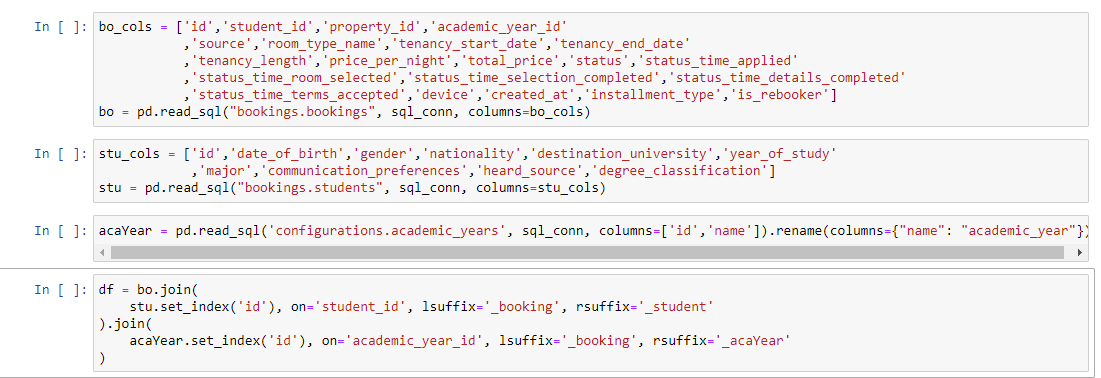
\includegraphics[width=10cm]{figures/joining_tables.png}
 \caption{Section of Jupiter Notebook for data cleaning where I joined 3 sql tables into 1 dataframe using there respective id's}
\end{figure}

With all of the necessary data stored in the data warehouse I imported the relevant tables into a Jupiter Notebook to perform the data cleaning stages. My aim is to include only valid bookings that made it the whole way through the booking process and then separate into cancelled or not. I started by removing any booking in the dataset that didn't have a total price or with a total price less than 1 as this meant the booking was not stored in the system correctly and may have been used for testing. I then removed any booking that did not get to the terms accepted stage since this could not be treated as a cancellation or a booking as the customer process was not finished.

\begin{figure}[hbt!]
 %\centering
 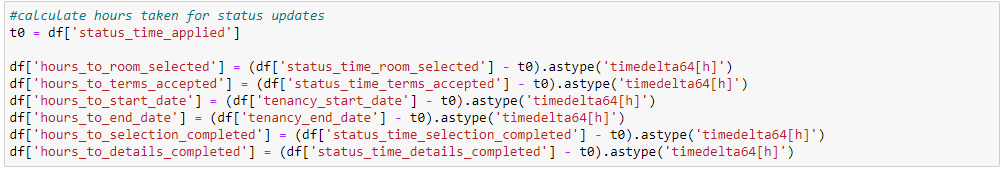
\includegraphics[width=10cm]{figures/time_variables.png}
 \caption{Section of Jupiter Notebook for data cleaning for creating features from the dataset by measuring the time taken to complete each stage of the booking process in the number of hours from the start date}
\end{figure}

Using the status time applied column to act as the first point where the booking process was started I created attributes used to store how long the customer took within each stage of the booking process as this may be able to indicate weather or not the user will cancel there booking.  \textbf{find a reference to support this}.

To account for the missing values in some of the categorical columns I use the pandas fill na method to replace the null values with Other  to prevent errors from occurring during the modeling stages when trying to handle null values.

\section{Modeling}

I used Azure ML Studio to evaluate and compare multiple different algorithms. ML studio is a cloud environment used to train, deploy, automate, manage and track ML models. It can be used for multiple different types of machine learning like supervised or unsupervised and deep learning. It gives the ability to write code in Python, R and its own no-code environment.  I used the cloud Jupiter notebook features for the data cleaning and preparation stages as well as testing models. To evaluate and compare multiple different algorithms I used Automated ML through its Python SDK on my cleaned dataset. Doing this meant I was able to test a large variation of regression algorithms.

I used a train test split of 20 percent test size with the sklearn model selection library. why did I used 20 percent

\begin{figure}[hbt!]
 %\centering
 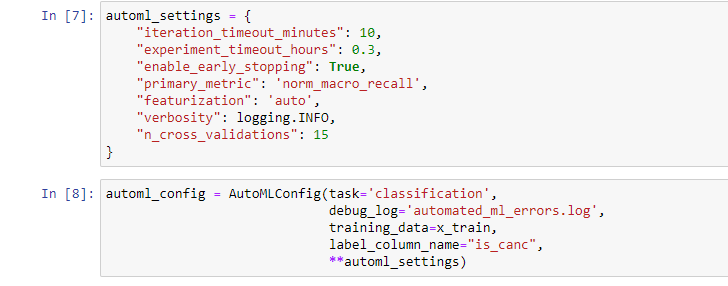
\includegraphics[width=10cm]{figures/auto_ml_settings.png}
 \caption{AutoML config settings for running classification algorithm}
\end{figure}

Running the algorithm is setup using the AutoMLConfig class in the Azure ML python SDK, the object contains all of the parameters used for configuring the experiment run. for a classification algorithm the task attribute is set to classification along with passing the training data and the target column label. Setting the number of cross validations to 15 means AutoML will run 15 different classifications on the training data outputting the results of each iteration. This output is then ranked by the selected primary metric which I have selected as norm macro recall, AzureML optimises models selected based on the primary metric. 

Using the featurization auto setting allows Azure ML to automatically detect the column types and apply the optimal data preprocess techniques, for categorical data the One Hot encoding technique is applied to create a new variable for each stage of the categorical attribute represented as binary. The process of featurization is able to detect columns with high cardinality.  High cardinality means a attribute contains a large number of unique values, this was true for columns destination university, major and nationality this is an expected result as the dataset contains students from a large variety of university's and nationalities. The problem with this is when applying the One Hot encoding technique each unique value increases the dimensionality of the feature matrix having the potential to result in model over fitting.

After the configuration is setup it can be passed to the Experiment.submit class, In this case I used the local run configuration so the cloud resources were not consumed running many iterations of the classification model. As each model is generated its results are outputted to the screen

\section{Evaluation}

\begin{itemize}
\item give a brief intro of evaluating the results
\end{itemize}


\section{Deployment}

\begin{itemize}
\item intro of how this will be deployed using azure
\end{itemize}



